\documentclass[10pt,twocolumn,twoside,final]{IEEEtran}

% cite package, to clean up citations in the main text. Do not remove.
\usepackage{cite}
\usepackage{lastpage,fancyhdr,graphicx}
\usepackage{amssymb,amsmath}

\bibliographystyle{plain}

% Remove brackets from numbering in List of References
\makeatletter
\renewcommand{\@biblabel}[1]{\quad#1.}
\makeatother

% *** SUBFIGURE PACKAGES ***
\ifCLASSOPTIONcompsoc
  \usepackage[caption=false,font=footnotesize,labelfont=sf,textfont=sf]{subfig}
\else
  \usepackage[caption=false,font=footnotesize]{subfig}
\fi

\begin{document}

\title{An Effective Model of HL-60 Differentiation}


% author names and affiliations
% use a multiple column layout for up to three different
% affiliations
\author{\IEEEauthorblockN{Ryan Tasseff\IEEEauthorrefmark{1},
Holly Jensen\IEEEauthorrefmark{1},
Johanna Congleton\IEEEauthorrefmark{2},
Andrew Yen\IEEEauthorrefmark{2},
Jeffrey D. Varner\IEEEauthorrefmark{1}}\\
\IEEEauthorblockA{\IEEEauthorrefmark{1}School of Chemical and Biomolecular Engineering,
Cornell University, Ithaca, NY 14850 USA}
\IEEEauthorblockA{\IEEEauthorrefmark{2}Department of Biomedical Sciences, Cornell University, Ithaca, NY 14850 USA}
\thanks{Manuscript received December 1, 2012; revised September 17, 2014.
Corresponding author: J. Varner (email:jdv27@cornell.edu).}}


%One of the defining features of this program is slowly induced, persistent MAPK activation.
%The molecular mechanisms of ATRA-induced commitment, arrest and functional differentiation are only partially understood.
%In this study, we explored the ATRA-inducible c-Raf, also known as Raf1 (Raf),
%interactome to determine the functional and regulatory architecture responsible for persistent MAPK activation in HL-60 cells.
%We surveyed a panel of 19 possible Raf interaction partners in the presence or absence of ATRA and the Raf inhibitor GW5074.
%We found five proteins (Akt, CK2, 14-3-3, Src and Vav1) that interacted with Raf under different conditions.
%In particular, the interaction between Raf and Vav1 demonstrated a relationship with ATRA-inducible MAPK activation and aspects of functional differentiation.

%this hypothesis using a combination of experimental and computational tools.
%First, we explored the  Raf interactome
%by surveying a panel of 19 possible binding partners using immunoprecipitation (IP),
%with and without ATRA and the Raf inhibitor GW5074.
%Initially, we expected increased ATRA-dependent association between Raf and kinases linked to BLR1 activity;
%however, this was not supported by data.
%Instead, we found that the interaction between the guanine nucleotide exchange factor Vav1 and Raf was both ATRA-inducible and simultaneously sensitive to Raf inhibition.
%Next, we considered how MAPK activation and differentiation were affected by the inhibition of Raf kinase activity in the presence and absence of ATRA.
%We showed that Raf activity was directly proportional to ERK phosphorylation and to functional differentiation processes such as the generation of reactive oxygen species (ROS).
%Moreover, interactions between Raf and kinase partners such as Akt or CK2, or the scaffolding protein 14-3-3 were largely insensitive to ATRA treatment.
%These studies established the working hypothesis that Vav1 (or potentially other ATRA-inducible proteins) acted as
%limiting members of a constitutively assembled trigger complex that propelled sustained MAPK activation, arrest and differentiation.
%We tested this hypothesis by constructing a mechanistic mathematical model of the Raf-Vav1 circuit,
%based on the IP and Western blot data presented in this study,
%and from previous literature.
%Interestingly, cells treated with ATRA for time periods shorter than the commitment phase retain a limited inheritable memory,
%which reduces the time required to reach commitment during subsequent ATRA exposure \cite{YEN1984}.

\maketitle

\begin{abstract}
Lessons learned in differentiation models, such as the lineage-uncommitted human myeloblastic cell line HL-60,
inform the analysis of more complex programs important to therapeutic applications.
In this study, we developed a minimal model of the All-Trans Retinoic Acid (ATRA) differentiation circuit of HL-60.
The minimal model encoded the positive feedback between an ATRA-inducible
membrane localized signalsome complex and mitogen-activated protein kinase (MAPK) activation.
We estimated an ensemble of model parameters using measurements from ATRA-induced HL-60 differentiation,
and tested the model in experimentally perturbed HL-60 cells.
Bifurcation analysis of this model predicted bistability in ppERK levels as a function of ATRA forcing.
A functional consequence of this was the ability to lock the MAPK cascade into a self-sustaining activated state, even after ATRA removal.
These simulations were then qualitatively validated with ATRA washout experiments.
The minimal model, despite its simplicity, captured the key features of the ATRA response of HL-60 cells such as
sustained MAPK activation, the impact of gene deletion and kinase inhibition.
\end{abstract}


\begin{IEEEkeywords}
Differentiation, mathematical modeling, bifurcation analysis.
\end{IEEEkeywords}

%If differentiation programs could be rationally manipulated, regenerative treatments might be possible for cancers, spinal cord injuries and neurodegenerative disorders.
%However, we must first understand the organization and operation of these programs \cite{Young2011}.

\section{Introduction}
Understanding differentiation,
the process by which precursor cells become more specialized cell types, is an important challenge.
Lessons learned in differentiation models, such as the lineage-uncommitted human myeloblastic cell line HL-60,
informs our analysis of more complex programs important to therapeutic applications.
HL-60 has been a durable experimental differentiation model since the late 1970's \cite{Breitman1980}.
HL-60 undergoes cell cycle arrest and either myeloid or monocytic differentiation following stimulation.
All-Trans Retinoic Acid (ATRA) induces G1/G0-arrest and myeloid differentiation in HL-60 cells,
while 1,25-dihydroxy vitamin D3 induces arrest and monocytic differentiation.
Commitment to cell cycle arrest and terminal differentiation requires approximately 48 hr of treatment,
during which HL-60 cells undergo two division cycles.

\begin{figure}[!t]
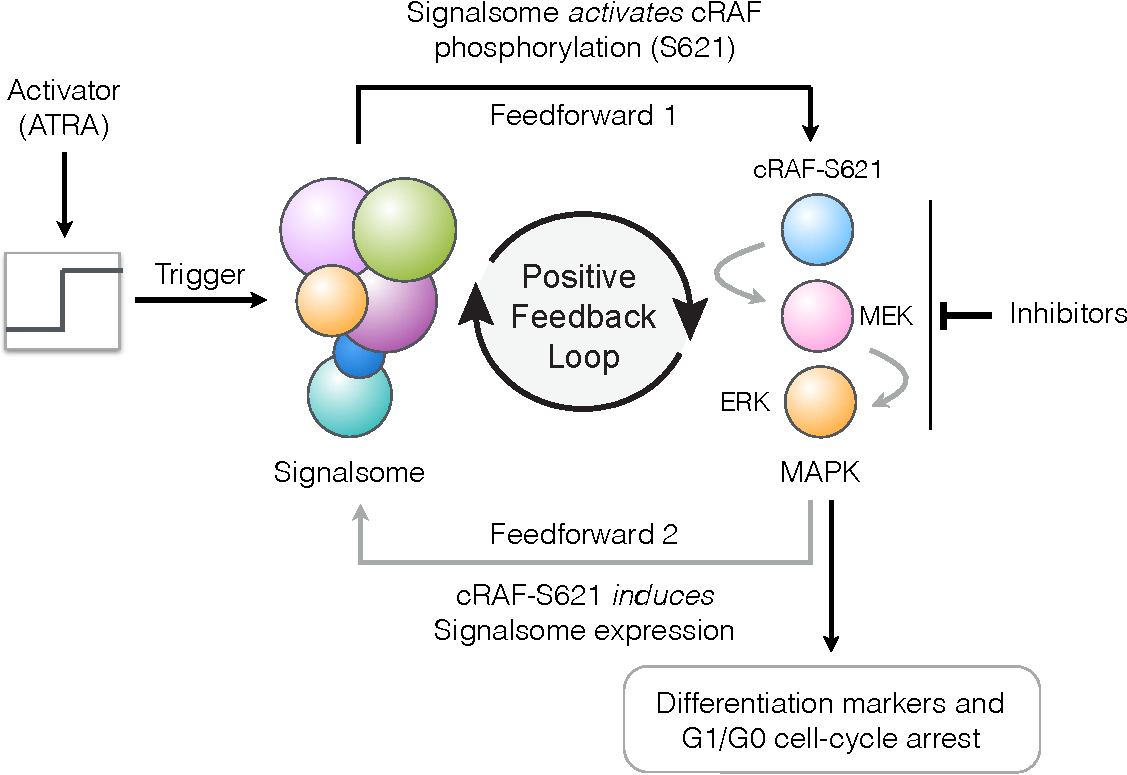
\includegraphics[width=0.5\textwidth]{./figs/Fig-1-Network.pdf}
\caption{Schematic of the reduced All-Trans Retinoic Acid (ATRA) differentiation circuit.
ATRA activates an upstream Trigger, which promotes the formation of the signalsome complex.
The signalsome activates the mitogen-activated protein kinase (MAPK) cascade.
MAPK then drives the downstream differentiation program and signalsome formation.}\label{fig:network}
\end{figure}

Sustained mitogen-activated protein kinase (MAPK) activation is a defining feature of ATRA-induced HL-60 differentiation.
ATRA drives sustained MEK-dependent activation of the RAF/MEK/ERK pathway, leading to arrest and functional differentiation \cite{Yen1998}.
MEK inhibition results in the loss of ERK and RAF phosphorylation, and the failure to arrest and terminally differentiate \cite{Yen1998,Hong2001}.
ATRA (and its metabolites) are ligands for the hormone activated nuclear transcription factors retinoic acid receptor (RAR) and retinoid X receptor (RXR) \cite{Mangelsdorf1990}.
Activation of RAR and RXR is necessary for ATRA-induced RAF phosphorylation and MAPK activation \cite{Hong2001}.
Transcription factor complexes involving RAR and RXR induce the expression of several proteins
including the putative heterotrimeric Gq protein-coupled receptor BLR1 \cite{WANG2004}.
BLR1, identified as an early ATRA (or D3)-inducible gene in HL-60 \cite{YEN1990},
is necessary for MAPK activation, growth arrest and functional differentiation \cite{WANG2004}.
Members of the BLR1 transcriptional activator complex, e.g. NFATc3 and CREB,
are phosphorylated by ERK, JNK or p38 MAPK family members suggesting positive feedback between BLR1 expression and MAPK activation \cite{Yang2002}.
BLR1 overexpression enhanced RAF phosphorylation and accelerated terminal differentiation.
BLR1 knock-out cells failed to activate RAF or differentiate in the presence of ATRA \cite{Wang2008}.
Lastly, RAF inhibition reduced BLR1 expression and functional differentiation \cite{Wang2008}.

Tasseff et al., hypothesized that BLR1-MAPK positive feedback was essential for ATRA-induced sustained MAPK activation,
cell cycle arrest and functional differentiation \cite{Tasseff2011}.
In this study, we tested this hypothesis by analyzing a minimal model of ATRA-inducible HL-60 differentiation (Fig. \ref{fig:network}).
The minimal model, composed of five differential equations, encoded the positive feedback between an ATRA-inducible
membrane localized signalsome complex and MAPK activation.
We estimated an ensemble of model parameters using measurements from ATRA-induced HL-60 differentiation,
and tested the model in experimentally perturbed HL-60 cells.
The minimal model, despite its relative simplicity, captured the key features of the ATRA response of HL-60 cells such as
sustained MAPK activation, the impact of gene deletion and kinase inhibition.

%based on a comprehensive mathematical model of ATRA-induced siganling

%\begin{figure*}[!t]
%	\centering
%	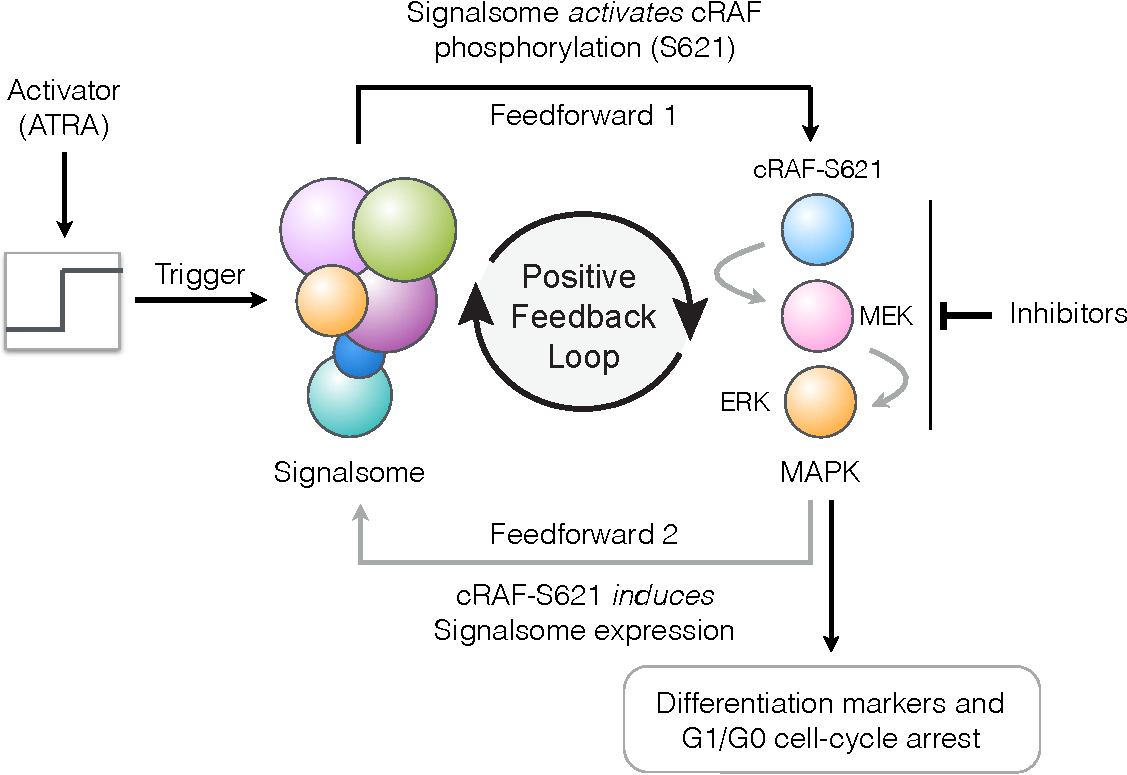
\includegraphics[width=\textwidth]{./figs/Fig-1-Network.pdf}
%	\caption{Schematic of the two component ATRA induced HL-60 differentiation circuit.}
%\end{figure*}

\begin{figure}[!t]\centering
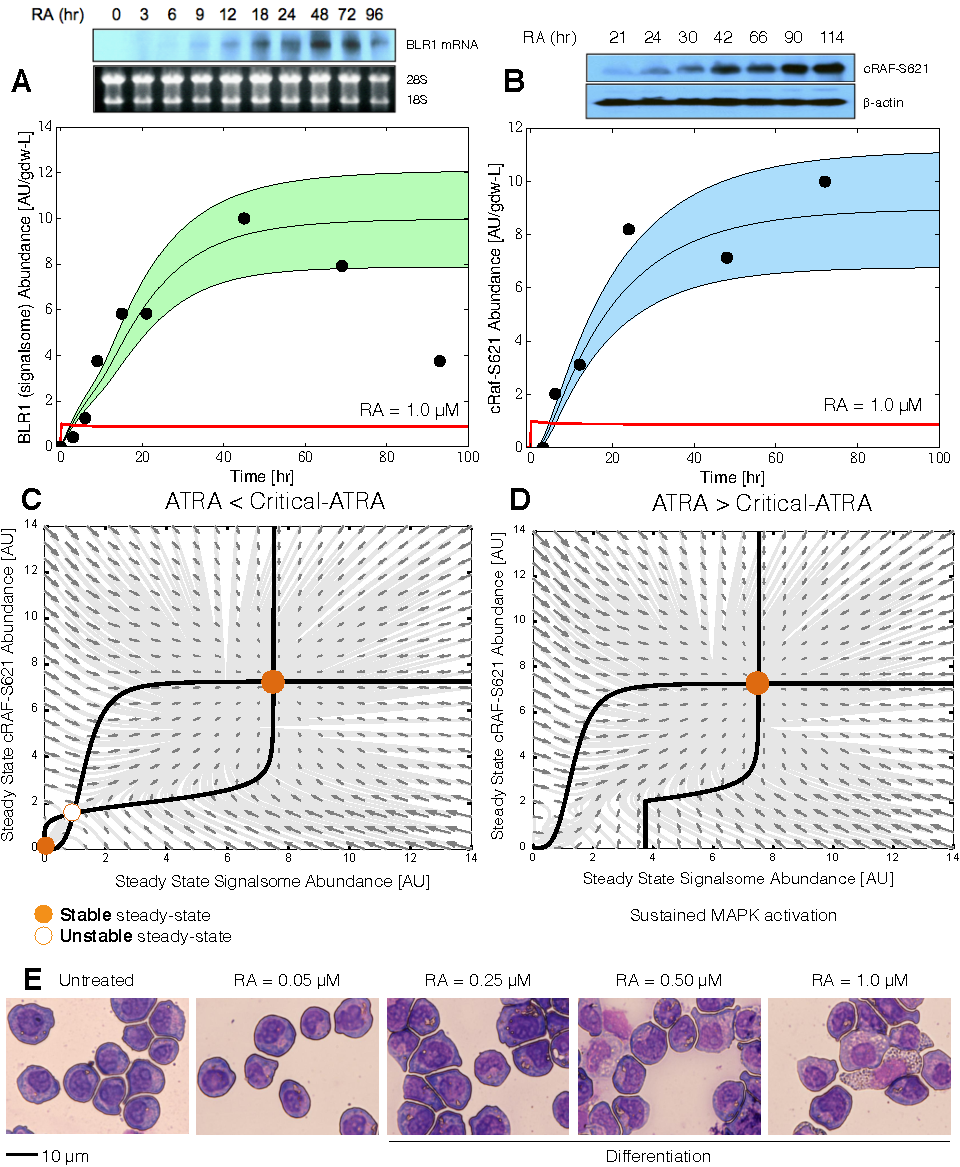
\includegraphics[width=0.50\textwidth]{./figs/Fig-2-cRaf-BLR1-Fit-Analysis.pdf}
\caption{Model analysis for ATRA-induced HL-60 differentiation.
A: BLR1 mRNA versus time following exposure to 1$\mu$M ATRA at t = 0 hr.
B: cRAF-S621 versus time following exposure to 1$\mu$M ATRA at t = 0 hr.
Points denote experimental measurements, solid lines denote the mean model performance. Shaded regions denote the 99\% confidence interval calculated over the parameter ensemble.
Qualitative analysis of the effective HL-60 differentiation model.
C: Signalsome and cRAF-S621 nullclines for ATRA below the critical threshold.
The reduced order model had two stable steady states and a single unstable state in this regime.
D: Signalsome and cRAF-S621 nullclines for ATRA above the critical threshold.
The reduced order model had only a single stable steady state in this regime.
E: HL-60 morphological response to increasing ATRA concentration. }\label{fig:model-fitting}
\end{figure}

\section{Results}

The minimal signalsome-MAPK model recapitulated sustained activation following exposure to 1$\mu$M ATRA (Fig. \ref{fig:model-fitting}A-B).
An ensemble of minimal model parameter sets was estimated by minimizing the difference between simulations and time-series measurements of BLR1 mRNA (signalsome component) and activated cRAF phosphorylated at Serine 621 (cRAF-S621) following the addition of 1$\mu$M ATRA using particle swarm optimization (PSO). Each particle in the swarm contributed a member to the ensemble of parameter sets.
The minimal feedback architecture captured both ATRA-induced BLR1 expression (Fig. \ref{fig:model-fitting}A) and sustained phosphorylation of cRAF at Serine 621
in a growing population of HL-60 cells (Fig. \ref{fig:model-fitting}B).
However, the minimal architecture failed to capture the decline of BLR1 expression after 48 hr of ATRA exposure,
suggesting additional components were present in the ATRA-induced differentiation circuit.

The minimal signalsome-MAPK feedback circuit was bistable with respect to ATRA forcing (Fig. \ref{fig:model-fitting}C-D).
Bifurcation analysis predicted two stable steady-states and a single unstable state when ATRA was present below a critical threshold (Fig. \ref{fig:model-fitting}C).
In the lower stable state, neither the signalsome nor cRAF-S621 were present. Thus, the differentiation program was deactivated.
On the other hand, at the high stable state, both the signalsome and cRAF-S621 were present, indicating sustained activation and differentiation.
Interestingly, when ATRA was above the critical threshold, only the activated state was possible (Fig. \ref{fig:model-fitting}D).
Taken together, bifurcation analysis suggested qualitatively different behavior was possible depending upon the
degree of ATRA forcing. Below a critical threshold, both deactivated and activated behavior were possible, while above the threshold, only activated behavior was possible.
To test these findings, we first identified the ATRA threshold, by exposing HL-60 cells to different ATRA concentrations (Fig. \ref{fig:model-fitting}E).
Morphological changes associated with differentiation were visible for ATRA $\geq$ 0.25 $\mu$M, suggesting the critical ATRA
threshold was near this concentration.

%\begin{figure}[!t]\centering
%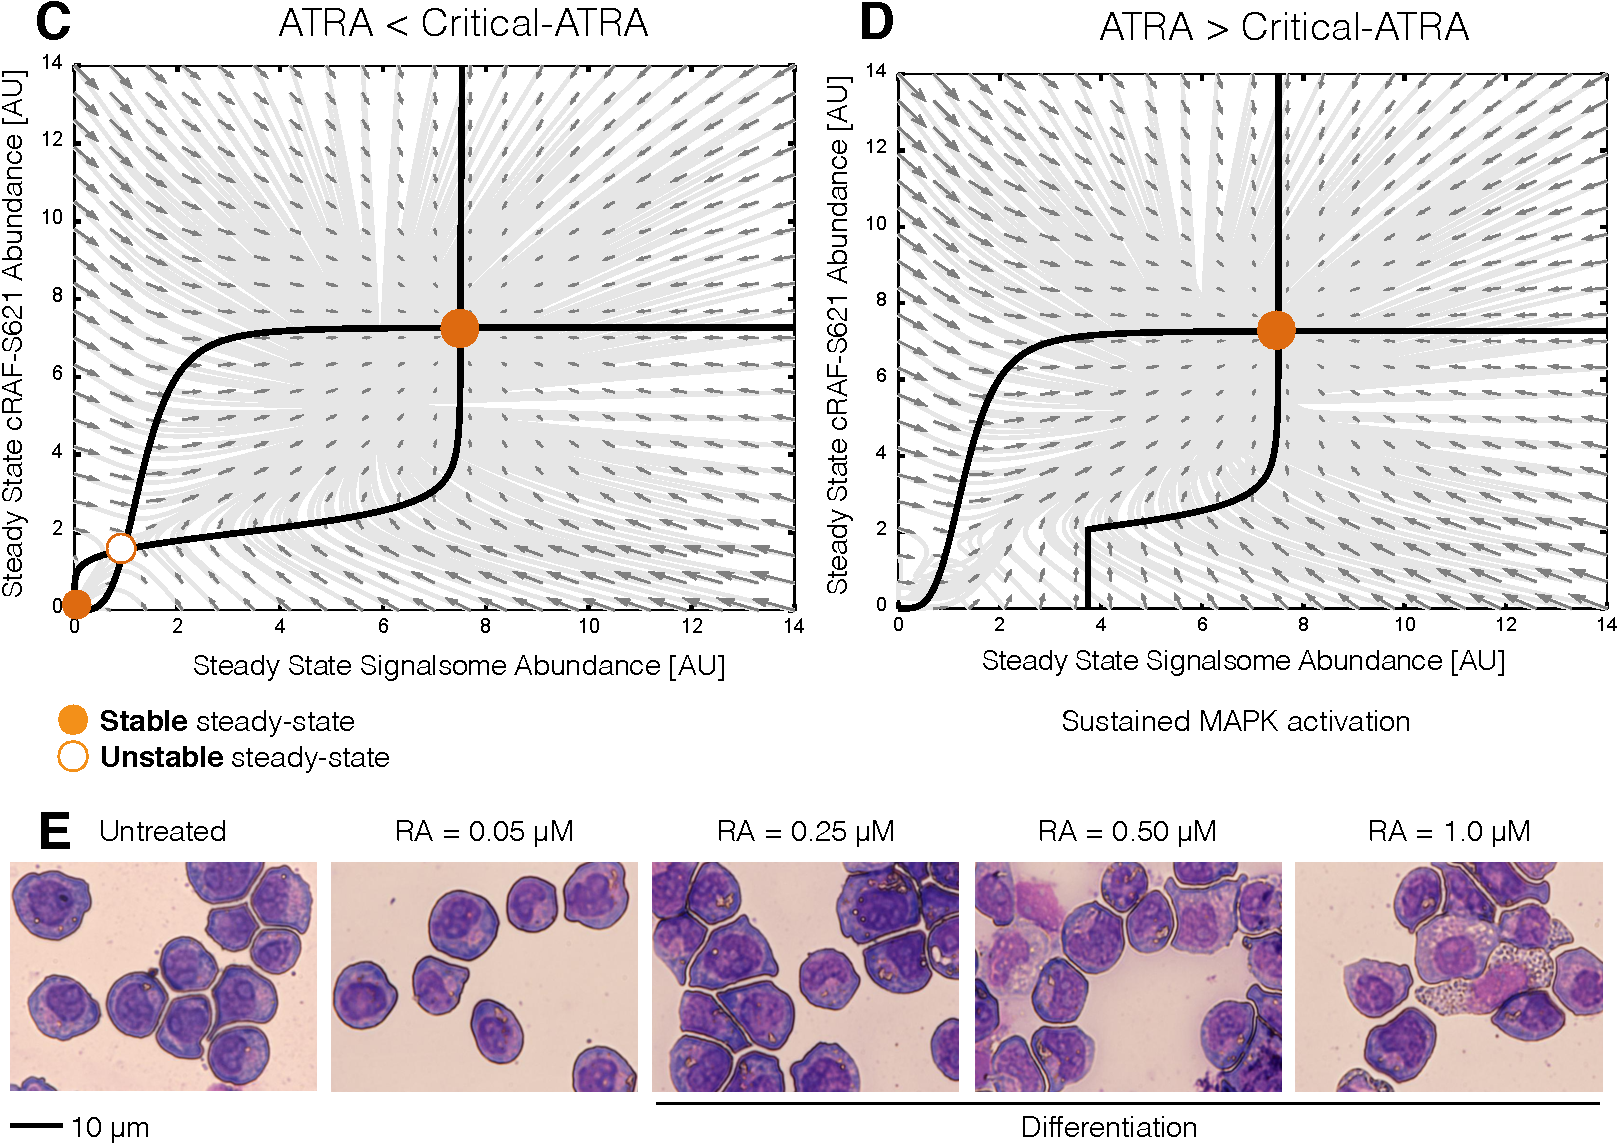
\includegraphics[width=0.5\textwidth]{./figs/Fig-3-QualitativeBehavior.pdf}
%\caption{Qualitative analysis of the effective HL-60 differentiation model. A: Signalsome and cRAF-S621 nullclines for ATRA below the critical limit. The reduced order model has two stable steady states and a single unstable state in this regime. B: Signalsome and cRAF-S621 nullclines for ATRA above the critical limit. The reduced order model has only a single stable steady state in this regime. C: HL-60 morphological response to increasing ATRA concentration. }\label{fig:bifurcation-results}
%\end{figure}

The minimal model recapitulated molecular perturbations to the ATRA-induced positive feedback circuit (Fig. \ref{fig:model-predictions}).
Self sustaining activation resulted from reinforcing positive feedback between the signalsome and MAPK.
Thus, if we inhibited or removed elements from the minimal circuit we expect the siganlsome and MAPK signals to decay.
We tested this hypothesis by simulating ATRA induced activation in the presence of kinase inhibitors and with key circuit elements removed (Fig. \ref{fig:model-predictions}).
Consistent with previous experimental results using multiple MAPK inhibitors, ATRA activation in the presence of MAPK inhibitors lowered the steady-state value of signalsome (Fig. \ref{fig:model-predictions}A). BLR1 deletion removed the ability of the circuit to maintain a sustained MAPK response following the withdraw of ATRA (Fig. \ref{fig:model-predictions}B, gray). On the other hand, in the presence of BLR1, the cRAF-S621 signal was maintained following the withdraw of ATRA, demonstrating the self sustaining nature of the circuit (Fig. \ref{fig:model-predictions}B, blue). Washout experiments in which cells were exposed to 1.0$\mu$M ATRA for 24 hr, and then transferred to fresh media without ATRA, confirmed the persistence of the self sustaining activated state for up to 144 hr (Fig. \ref{fig:model-predictions}C). However, beyond 144 hr the activated MAPK signal (as measured by phosphorylated ERK1/2) decayed. The decreasing MAPK signal indicated additional factors and connections were likely involved in the ATRA circuit beyond the signalsome and MAPK.

\section{Discussion}
We presented a minimal model of ATRA-inducible differentiation of HL-60 cells.
The minimal model, composed of five differential equations, encoded the positive feedback between the ATRA-inducible
membrane localized signalsome and the MAPK pathway.
We estimated an ensemble of model parameters using measurements of siganlsome and MAPK components following ATRA induction in HL-60 using particle swarm optmization.
We then tested the model ensemble using data generated in experimentally perturbed HL-60 cells.
The minimal model captured the key features of the ATRA response such as
sustained MAPK activation, the impact of gene deletion and kinase inhibition, despite its relative simplicity.
Taken together, this study provided further details on sustained MAPK activation, mechanistic insight into cellular memory,
and proof-of-concept that a combination of experimental and computational methods is an effective strategy for dissecting complex intracellular signaling programs.

The performance of the minimal ATRA model was impressive given its limited size. However, there were several issues that could be further explored.
First, the choice of max/min integration rules or the particular form of the transfer functions could be generalized to include other rule types and functions.
Theoretically, an integration rule is a function whose domain is a set of transfer function inputs, and whose range is $v\in[0,1]$.
Thus, integration rules other than max/min could be used, such as the mean or the product, assuming the range of the transfer functions is always $f\in[0,1]$.
Alternative integration rules such as the mean might have different properties which could influence model identification or performance.
For example, a mean integration rule would be differentiable, which allows derivative-based optimization approaches to be used.
The particular form of the transfer function could also be explored. We choose a Hill-like function because of its
prominence in the systems and synthetic biology community. However, the only mathematical requirement for a transfer function is that it map a non-negative continuous or categorical variable into the range $f\in[0,1]$. Thus, many types of transfer functions are possible.

\section{Materials and Methods}

\begin{figure}[!t]\centering
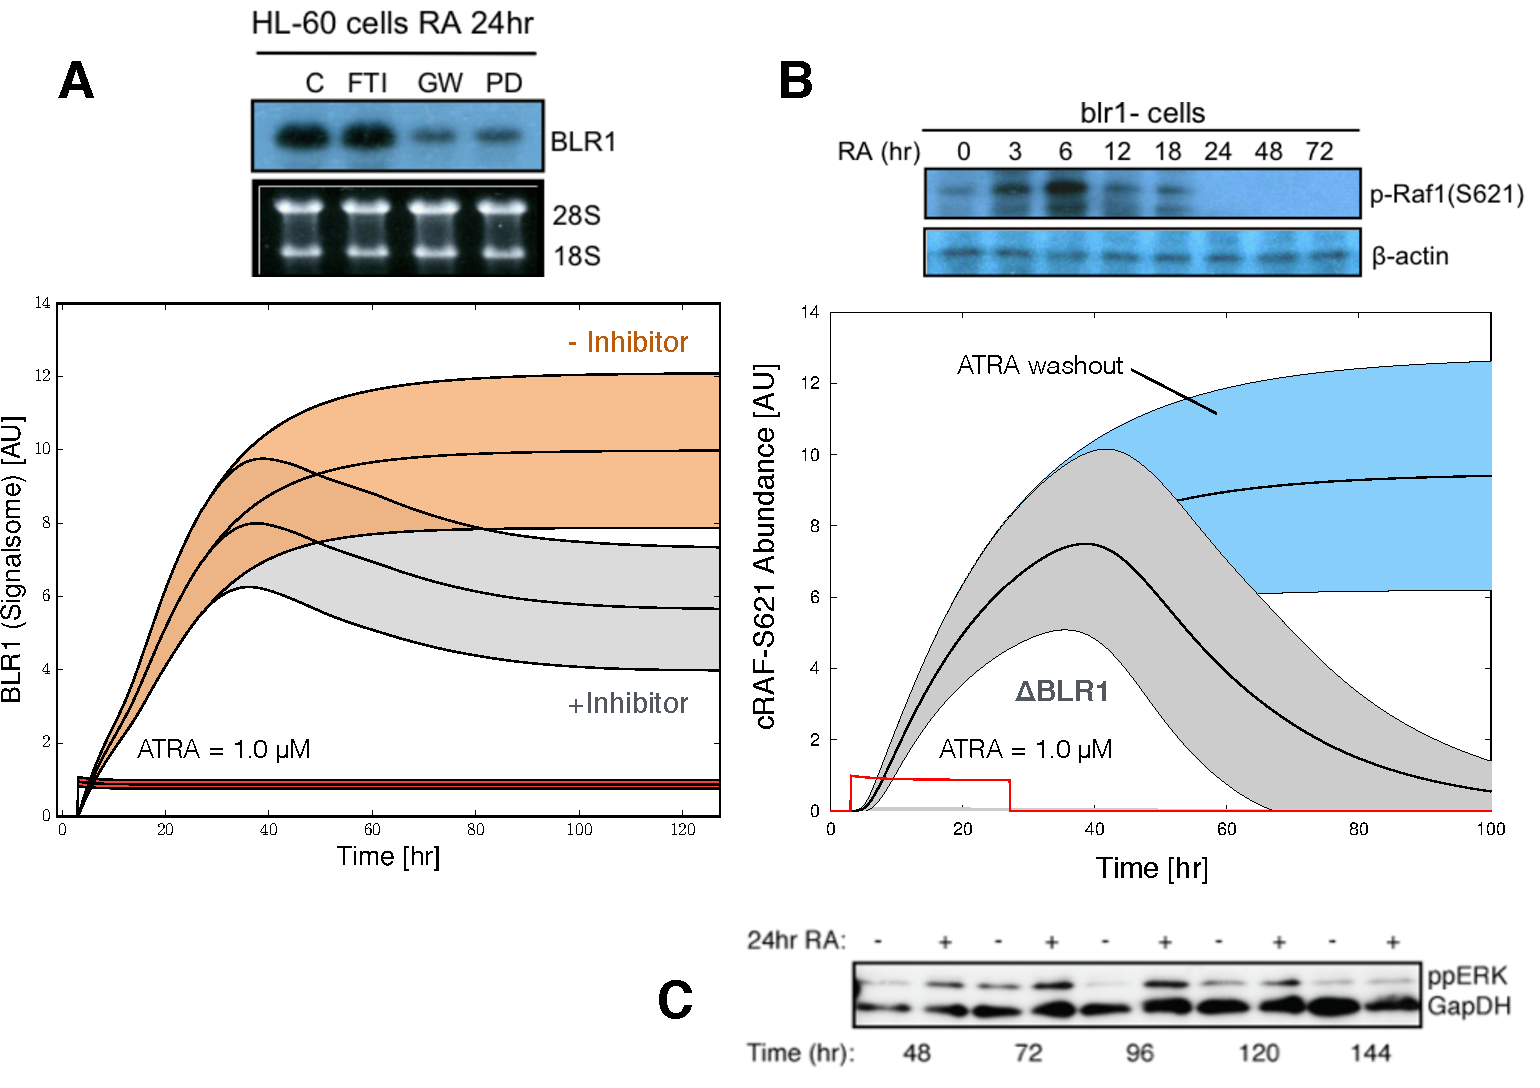
\includegraphics[width=0.50\textwidth]{./figs/Fig-4-Predictions.pdf}
\caption{Model simulation versus experimental data for BLR1 and activated cRAF following ATRA stimulation in HL-60 cells. A: BLR1 mRNA versus time following exposure to 1.0$\mu$M ATRA with and without kinase inhibitor. B: cRAF-S621 versus time following exposure to 1.0$\mu$M ATRA at t = 3 hr and removal of ATRA at t = 24 hr. Blue region denotes the nominal model, while gray denotes ATRA and BLR1 removal. C: Western blot of phosphorylated ERK1/2 as a function of time in HL-60 cells following exposure to 1.0 $\mu$M ATRA at t = 0 hr and removal of ATRA at t = 24 hr. Points denote experimental measurements. The solid line denotes the mean model performance while the shaded regions denote the 99\% confidence interval calculated over the parameter ensemble. Experimental data in panels A and B were reproduced from Wang and Yen \cite{Wang2008}, data in panel C is reported in this study. }\label{fig:model-predictions}
\end{figure}

\noindent\subsubsection*{Minimal model equations}
We modeled the minimal ATRA differentiation circuit using a hybrid approach which integrated ordinary differential equations with logical rules \cite{pr3010138}.
This approach allowed mechanistic detail, which normally increases the dimension and complexity of the model equations, to be encoded by logical transfer functions, thereby significantly reducing the model dimension. Let the abundance of species $i$ ($x_{i}$) in the model be described by:
\begin{equation}
	\frac{dx_{i}}{dt}  =  \sum_{j = 1}^{\mathcal{R}}\sigma_{ij}r_{j}\left(\mathbf{x},\mathbf{k}\right) - \left(\mu+k_{d,i}\right)x_{i}\qquad{i=1,\hdots,\mathcal{M}}\\
\end{equation}
where $\mathcal{R}$ denotes the number of reactions in the model, and $\mathcal{M}$ denotes the number of species in the model.
The quantity $r_{j}\left(\mathbf{x},\mathbf{\epsilon},\mathbf{k}\right)$ denotes the rate of reaction $j$.
Typically, reaction $j$ is a non-linear function of biochemical species abundance and unknown kinetic parameters $\mathbf{k}$ ($\mathcal{K}\times{1}$).
The quantity $\sigma_{ij}$ denotes the stoichiometric coefficient for species $i$ in reaction $j$.
If $\sigma_{ij}>0$, species $i$ is produced by reaction $j$, if $\sigma_{ij}<0$, species $i$ is consumed by reaction $j$,
while $\sigma_{ij} = 0$ indicates species $i$ is not connected with reaction $j$.
Material balances were subject to the initial conditions $\mathbf{x}\left(t_{o}\right) = \mathbf{x}_{o}$.

Each reaction rate was written as the product of two terms, a kinetic term ($\bar{r}_{j}$) and a control term ($v_{j}$):
\begin{equation}\label{eqn:rate-factor}
	r_{j}\left(\mathbf{x},\mathbf{\epsilon},\mathbf{k}\right) = \bar{r}_{j}v_{j}
\end{equation}
In this study, we used either zero- or first-order kinetics.
The control term $0\leq v_{j}\leq 1$ depended upon the combination of factors which influenced the activity of species $i$.
For each node, we used a rule-based approach to select from competing control factors.
If a node j was influenced by $1,\dots,m$ possible factors, we modeled this relationship as:
\begin{equation}
	v_{j} = \mathcal{I}_{j}\left(f_{1j}\left(\mathcal{Z}\right),\hdots,f_{mj}\left(\mathcal{Z}\right)\right)
\end{equation}where $0\leq f_{ij}\left(\mathcal{Z}\right)\leq 1$ was a regulatory transfer function that quantified the influence of node $i$ on the activity of node $j$.
The function $\mathcal{I}_{j}\left(\cdot\right)$ denotes an integration rule which maps the output of each of the regulatory transfer functions into the overall control
variable for process j.
If a process has no modifying factors, $v_{j} = 1$.
While there are many possible forms for $f_{ij}\left(\mathcal{Z}\right)$, in this study, each regulatory transfer function took the form:
\begin{equation}\label{eqn:control-factor}
	f_{i}\left(\mathcal{Z}_{j},k_{ij}\right) = k_{ij}^{\eta}\mathcal{Z}_{j}^{\eta}/\left({1 + k_{ij}^{\eta}\mathcal{Z}_{j}^{\eta}}\right)
\end{equation}where $\mathcal{Z}_{j}$ denotes the abundance of the $j$ factor (e.g., metabolite or protein abundance), and $k_{ij}$ and $\eta$ are control parameters.
The parameter $k_{ij}$ was a gain parameter, while $\eta$ was a cooperatively parameter.
In this study, we used $\mathcal{I}_{j}\in\left\{\max,\min\right\}$ as shown in Wayman et al., \cite{pr3010138}.

\noindent\subsubsection*{Estimation of model parameters}
Model parameters were estimated by minimizing the squared difference between simulations and experimental data taken from ATRA-induced HL-60 cells:
\begin{equation}\label{eqn:objective-function}
	E_{j}(\mathbf{k}) = \sum_{i=1}^{\mathcal{T}_{j}}\biggl(\hat{\mathcal{M}}_{ij}-\hat{y}_{ij}(\mathbf{k})\biggr)^2 + \left(\frac{{\mathcal{M}^{\prime}_{ij}}-\max{y_{ij}}}{{\mathcal{M}^{\prime}_{ij}}}\right)^{2}
\end{equation}
The terms $\hat{\mathcal{M}}_{ij}$ and $\hat{y}_{ij}$ denote scaled experimental observations and simulation outputs from training set $j$.
The quantity $i$ denoted the sampled time-index and $\mathcal{T}_{j}$ denoted the number of time points for experiment j.
The first term in Eqn. \eqref{eqn:objective-function} quantified the relative error in the simulation.
We used only immunoblot measurements for model training.
Thus, we trained the model on the \emph{relative} change between bands within each training data set.
The read-out from the training immunoblots was band intensity where we assumed intensity was only loosely proportional to concentration.
Suppose we have the intensity for species $x$ at time $\{t_{1},t_{2},..,t_{n}\}$ in condition $j$. The scaled-value $\hat{\mathcal{M}}_{ij}$ would then be given by:
\begin{equation}\label{norm_exp_data}
\hat{\mathcal{M}}_{ij} = \frac{\mathcal{M}_{ij} - \min_{i}\mathcal{M}_{ij}}{\max_{i}{\mathcal{M}_{ij}}-\min_{i}{\mathcal{M}_{ij}}}
\end{equation}
Under this scaling $0\leq\hat{\mathcal{M}}_{ij}\leq{1}$ where $\hat{\mathcal{M}}_{ij}=0$ describes the lowest intensity band and $\hat{\mathcal{M}}_{ij}=1$ describes the highest intensity band.
A similar scaling was defined for the simulation output. The second-term in the objective function ensured the proper concentration scale was estimated by the model.
In this study, we set the highest intensity band to $\mathcal{M}^{\prime}_{ij} = 10$ [AU] for all simulations.
We minimized the total model residual $\sum_{j}E_{j}$ using Particle swarm optimization (PSO) \cite{PSO}.
The particle swarm optimization routine was implemented in the Python programming language.


%Model parameters were estimated by minimizing the difference between simulations and experimental measurements (squared residual):
%\begin{equation}\label{eqn:objective-function}
%	\min_{\mathbf{k}} \sum_{\tau=1}^{\mathcal{T}}\sum_{j=1}^{\mathcal{S}}\left(\frac{\hat{x}_{j}\left(\tau\right) - x_{j}\left(\tau,\mathbf{k}\right)}{\omega_{j}\left(\tau\right)}\right)^{2}
%\end{equation}where $\hat{x}_{j}\left(\tau\right)$ denotes the measured value of species $j$ at time $\tau$, $x_{j}\left(\tau,\mathbf{k}\right)$ denotes the simulated
%value for species $j$ at time $\tau$, and $\omega_{j}\left(\tau\right)$ denotes the experimental measurement variance for species $j$ at time $\tau$.

\subsubsection*{Cell culture and treatment}
Human myeloblastic leukemia cells (HL-60 cells) were grown in a humidified atmosphere of 5\% CO$_2$ at 37$^{o}$C and maintained in RPMI 1640 from Gibco (Carlsbad, CA)
supplemented with 5\% fetal bovine serum from Hyclone (Logan, UT) and 1x antibiotic/antimicotic (Sigma, St. Louis, MO).
Cells were cultured in constant exponential growth as described previously \cite{Brooks1996}.
Experimental cultures were initiated at $0.1\times10^6$ cells/mL 24 hr prior to 1$\mu$M ATRA treatment;
if indicated, cells were also treated with GW5074 (2$\mu$M) 18 hr before ATRA treatment.
For the cell culture washout experiments, HL-60 cells were treated with ATRA for 24 hr,
washed 3x with prewarmed serum supplemented culture medium to remove ATRA exposure,
and reseeded in ATRA-free media as described.
Western blot analysis was performed at incremental time points after removal of ATRA.

\subsubsection*{Chemicals}
All-Trans Retinoic Acid (ATRA) from Sigma-Aldrich (St. Louis, MO) was dissolved in
100\% ethanol with a stock concentration of 5mM, and used at a final concentration of 1$\mu$M (unless otherwise noted).
The Raf inhibitor GW5074 from Sigma-Aldrich (St. Louis, MO) was dissolved in DMSO with a stock concentration of 10mM,
and used at a final concentration of 2$\mu$M.
HL-60 cells were treated with 2$\mu$M GW5074 with or without ATRA (1$\mu$M) at 0 hr.
This GW5074 dosage had a negligible effect on the cell cycle distribution, compared to ATRA treatment alone.

\subsubsection*{Immunoprecipitation and western blotting}
Approximately $1.2 \times 10^7$ cells were lysed using 400$\mu$L of M-Per lysis buffer from Thermo Scientific (Waltham, MA).
Lysates were cleared by centrifugation at 16,950 $\times$ g in a micro-centrifuge for 20 min at 4$^{o}$C.
Lysates were pre-cleared using 100$\mu$L protein A/G Plus agarose beads from Santa Cruz Biotechnology (Santa Cruz, CA) by
inverting overnight at 4$^{o}$C.  Beads were cleared by centrifugation and total protein concentration
was determined by a BCA assay (Thermo Scientific, Waltham, MA).  Immunoprecipitations were setup by bringing
lysate to a concentration of 1.0g/L in a total volume of 300$\mu$L (M-Per buffer was used for dilution).
The anti-Raf antibody was added at 3 $\mu$L.
A negative control with no bait protein was also used to exclude the direct interaction of proteins with the A/G beads.
After 1 hr of inversion at 4$^{o}$C, 20$\mu$L of agarose beads was added and samples were left
to invert overnight at 4$^{o}$C. Samples were then washed three times with M-Per buffer by centrifugation.
Finally proteins were eluted from agarose beads using a laemmli loading buffer.
Eluted proteins were resolved by SDS-PAGE and Western blotting.  Total
lysate samples were normalized by total protein concentration (20$\mu$g per sample)
and resolved by SDS-PAGE and Western blotting.  Secondary HRP bound antibody was used for visualization.
All antibodies were purchased from Cell Signaling (Boston, MA) with the exception of anti-p621 Raf which was purchased from Biosource/Invitrogen  (Carlsbad, CA), and
anti-pS338 Raf which was purchased from Santa Cruz Biotechnology (Santa Cruz, CA); anti-retinoblastoma from Zymed (South San Francisco, CA); and anti-CK2 from BD Biosciences (San Jose, CA).

% References -
\bibliography{Paper_v1}

\end{document}
